% Wide, two-column-spanning figure. Requires \usepackage{graphicx} in the preamble.
% Put uncertainty_method_cmp.pdf on the graphics path (e.g. \graphicspath{{figures/}}) or use a full path.
% Citation keys li2023iti / selfaware / falseqa are defined in docs/blade-method.bib.
\begin{figure*}[t]
  \centering
  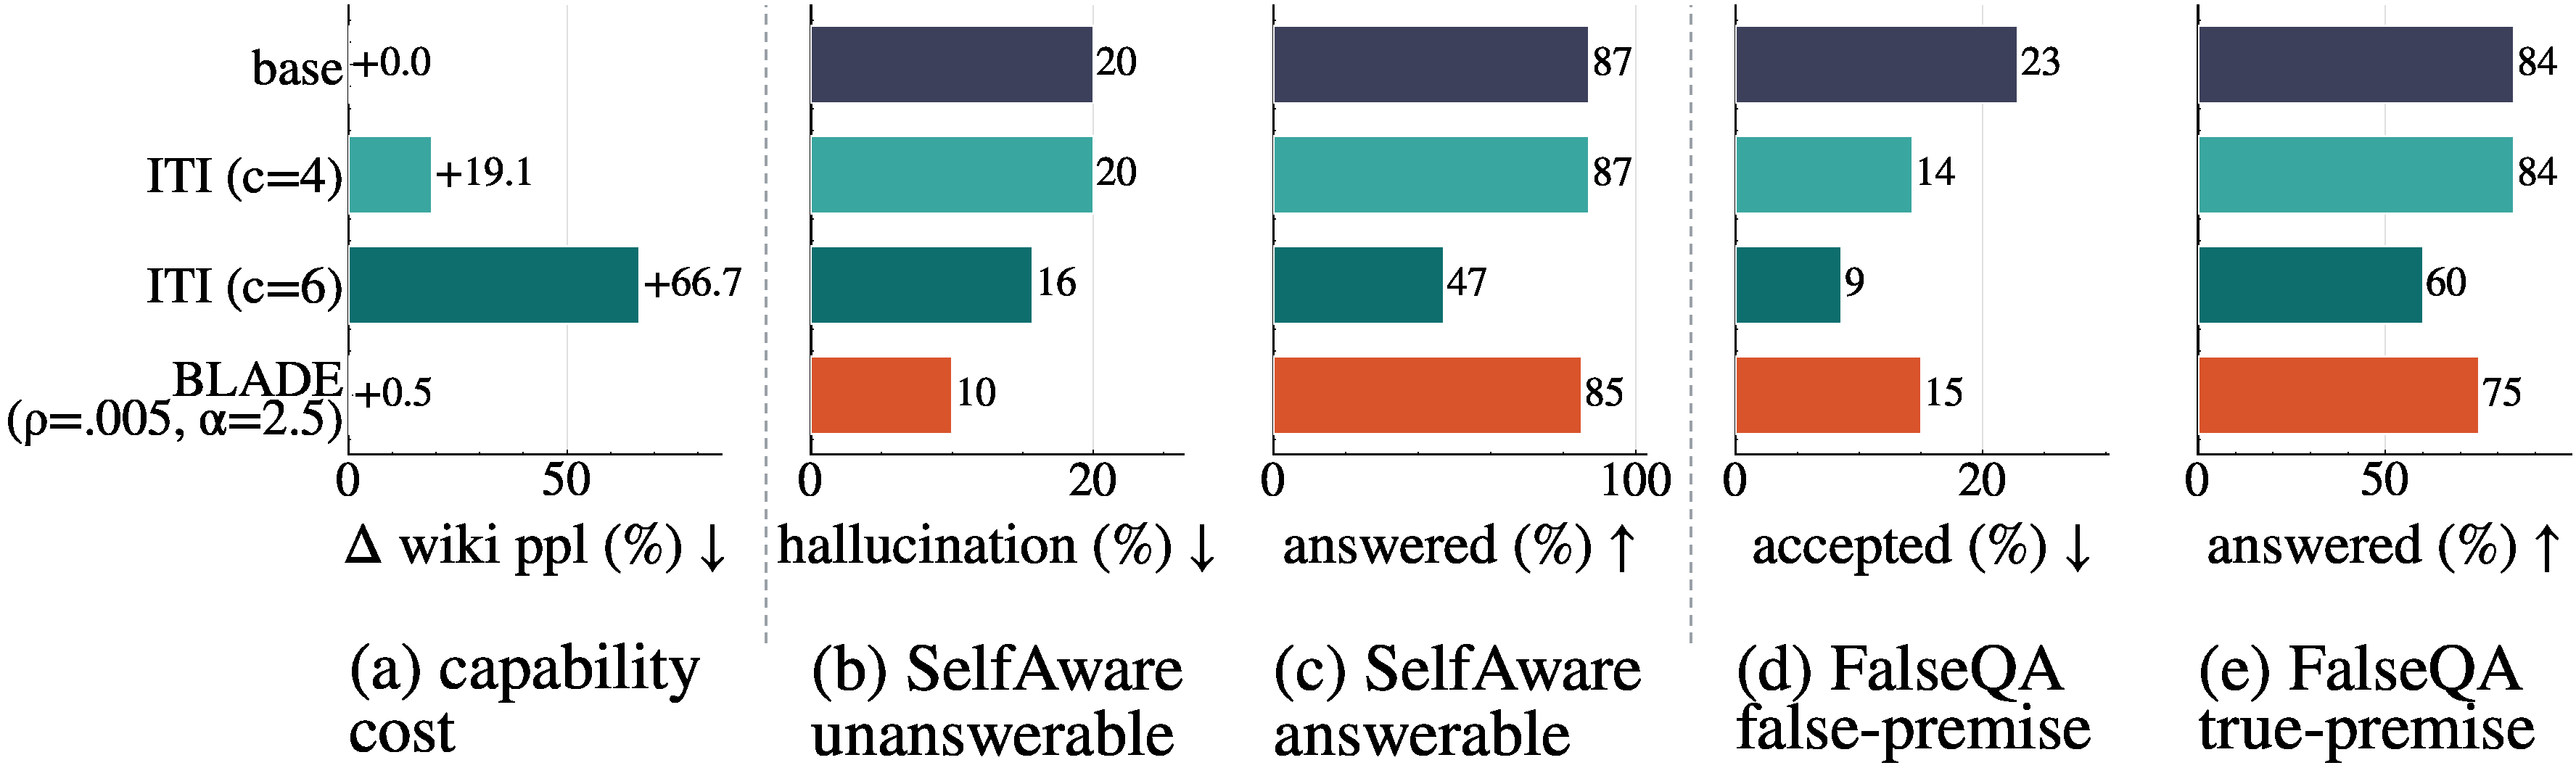
\includegraphics[width=\textwidth]{figures/uncertainty_method_cmp.pdf}
  \caption{%
    \textbf{Controlling closed-book epistemic (un)certainty on Qwen3-8B.}
    A single BLADE weight edit ($\rho\!=\!0.005$, $\alpha\!=\!2.5$) vs.\ ITI
    activation steering~\citep{li2023iti} at three strengths. Behavioral rates from a
    blind LLM judge; lower is better in (a,\,b,\,d), higher in (c,\,e).%
  }
  \label{fig:uncertainty-method-cmp}
\end{figure*}

% ---------------------------------------------------------------------------
% Body text (the "context" for the figure) — paste near the \ref, not in the caption.
% Dataset citations selfaware / falseqa are defined in docs/blade-method.bib.
% ---------------------------------------------------------------------------
\paragraph{Benchmarks.} We evaluate on two closed-book abstention benchmarks that probe
complementary failure modes. \textbf{SelfAware}~\cite{selfaware} pairs answerable
questions with \emph{unanswerable} ones---open scientific unknowns, under-specified or
subjective queries with no known answer. A calibrated model answers the former and
abstains on the latter; we therefore report the hallucination rate on the unanswerable
half and the answer rate on the answerable half. \textbf{FalseQA}~\cite{falseqa} pairs
questions built on a \emph{false premise} (a presupposition that is factually wrong) with
matched valid-premise questions. Here a calibrated model rejects or corrects the false
premise rather than answering as if it held; we report false-premise acceptance and
true-premise answering. Together they separate two kinds of epistemic humility: knowing
what is unknowable (SelfAware) and refusing a false presupposition (FalseQA).

Figure~\ref{fig:uncertainty-method-cmp} compares our BLADE weight edit against ITI
activation steering~\citep{li2023iti} on closed-book epistemic (un)certainty in Qwen3-8B.
Both methods are fit on the \emph{same} certain/uncertain prompt contrast at the last
prompt token, so the comparison isolates the mechanism---a sparse, static weight edit
versus per-head activation steering---rather than the direction source. All behavioral
rates are assigned by a blind LLM judge with the condition hidden. We report a single
BLADE operating point ($\rho\!=\!0.005$, $\alpha\!=\!2.5$; BLADE-G, thinking-off, layers
auto-selected) and ITI at steering strength $c\!\in\!\{2,4,6\}$ (in units of per-head
projection std; $c$ is ITI's dose, distinct from BLADE's amplification $\alpha$).

ITI reduces SelfAware unanswerable hallucination only at a strength that is catastrophic
for capability: it leaves this rate at the base $20\%$ for $c\!\in\!\{2,4\}$ and
lowers it to $16\%$ only at $c\!=\!6$, where C4 teacher-forced perplexity rises by
$57.3\%$ (panel~a) and answering on SelfAware answerable questions collapses to $47\%$
(panel~c). BLADE instead lowers unanswerable hallucination to $10\%$ (panel~b) while
holding perplexity essentially flat ($-0.3\%$) and preserving answering at $85\%$
(base $87\%$). On FalseQA false-premise acceptance (panel~d) the two methods are
comparable: BLADE reaches $15\%$ (base $23\%$), matched by ITI already at $c\!=\!2$
($16\%$, at only $+2.7\%$ perplexity) and beaten only by the capability-destroying
$c\!=\!6$ ($9\%$). BLADE also retains most true-premise answering ($75\%$ vs.\ base
$84\%$; panel~e). The distinguishing result is therefore SelfAware unanswerable
hallucination: BLADE is the only configuration that lowers it without a capability hit,
whereas ITI reduces it only at $c\!=\!6$, where perplexity and answering collapse.
